\documentclass[enabledeprecatedfontcommands,fontsize=12pt,paper=a4,twoside]{scrartcl}


\newcommand{\grad}{\ensuremath{^{\circ}} }
\renewcommand{\strut}{\vrule width 0pt height5mm depth2mm}

\usepackage{longtable}
\usepackage[utf8]{inputenc}
\usepackage[T1]{fontenc}
\usepackage[final]{pdfpages}
% obere Seitenränder gestalten können
\usepackage{fancyhdr}
\usepackage{moreverb}
% Graphiken als jpg, png etc. einbinden können
\usepackage{graphicx}
\usepackage[normalem]{ulem}
\useunder{\uline}{\ul}{}
\usepackage{stmaryrd}
% Floats Objekte mit [H] festsetzen
\usepackage{float}
% setzt URL's schön mit \url{http://bla.laber.com/~mypage}
\usepackage{url}
% Externe PDF's einbinden können
\usepackage{pdflscape}
% Verweise innerhalb des Dokuments schick mit " ... auf Seite ... "
% automatisch versehen. Dazu \vref{labelname} benutzen
\usepackage[ngerman]{varioref}
\usepackage[ngerman]{babel}
\usepackage{ngerman}
% Bibliographie
\usepackage{bibgerm}
% Tabellen
\usepackage{tabularx}
\usepackage{supertabular}
\usepackage[colorlinks=true, pdfstartview=FitV, linkcolor=blue,
            citecolor=blue, urlcolor=blue, hyperfigures=true,
            pdftex=true]{hyperref}
\usepackage{bookmark}
\usepackage{rotating}
\usepackage{float}

\hyphenation{Arbeits-paket}

% Damit Latex nicht zu lange Zeilen produziert:
\sloppy
%Uneinheitlicher unterer Seitenrand:
%\raggedbottom

% Kein Erstzeileneinzug beim Absatzanfang
% Sieht aber nur gut aus, wenn man zwischen Absätzen viel Platz einbaut
\setlength{\parindent}{0ex}

% Abstand zwischen zwei Absätzen
\setlength{\parskip}{1ex}

% Seitenränder für Korrekturen verändern
\addtolength{\evensidemargin}{-1cm}
\addtolength{\oddsidemargin}{1cm}

\bibliographystyle{gerapali}

% Lustige Header auf den Seiten
  \pagestyle{fancy}
  \setlength{\headheight}{70.55003pt}
  \fancyhead{}
  \fancyhead[LO,RE]{Software--Projekt 2\\ WiSe 2019/2020
  \\Architekturbeschreibung}
  \fancyhead[LE,RO]{Seite \thepage\\\slshape \leftmark\\\slshape \rightmark}

%Unicode Minuszeichen deklarieren, um es nicht überall austauschen zu müssen
\DeclareUnicodeCharacter{2212}{-}

%
% Und jetzt geht das Dokument los....
%

\begin{document}

% Lustige Header nur auf dieser Seite
  \thispagestyle{fancy}
  \fancyhead[LO,RE]{ }
  \fancyhead[LE,RO]{Universität Bremen\\FB 3 -- Informatik\\
  Prof. Dr. Rainer Koschke \\TutorIn: Marcel Steinbeck}
  \fancyfoot[C]{}

% Start Titelseite
  \vspace{3cm}

  \begin{minipage}[H]{\textwidth}
  \begin{center}
  \bf
  \Large
  Software--Projekt 2 WiSe 2019/2020\\
  \smallskip
  \small
  VAK 03-BA-901.02\\
  \vspace{3cm}
  \end{center}
  \end{minipage}
  \begin{minipage}[H]{\textwidth}
  \begin{center}
  \vspace{1cm}
  \bf
  \Large Benutzerhandbuch\\ Data Colorado\\
  \vfill
  \end{center}
  \centering
  
\includegraphics[width=0.4\textwidth]{UML/Logo.png}\\
  \end{minipage}
  \vfill
  \begin{minipage}[H]{\textwidth}
  \begin{center}
  \sf
  \begin{tabular}{lr}
  Liam Hurwitz & hurwitz@tzi.de \\
  Kevin Santiago Rodriguez Rey & kev\textunderscore rey@tzi.de \\
  Fabian Kehlenbeck & fkehlenb@tzi.de \\
  Aaron Rudkowski & rudkowsk@tzi.de \\
  Samuel Nejati Masouleh & samnej@tzi.de \\
  Leonard Haddad & s\textunderscore xsipo6@tzi.de \\  
\end{tabular}
  \\ ~
  \vspace{2cm}
  \\
  \it Abgabe: 08.03.2020 --- Version 1.0\\ ~
  \end{center}
  \end{minipage}

% Ende Titelseite

% Start Leerseite

\newpage

  \thispagestyle{fancy}
  \fancyhead{}
  \fancyhead[LO,RE]{Software--Projekt \\  2019/2020
  \\Benutzerhandbuch}
  \fancyhead[LE,RO]{Seite \thepage\\\slshape \leftmark\\~}
  \fancyfoot{}
  \renewcommand{\headrulewidth}{0.4pt}
  \tableofcontents

\newpage

  \fancyhead[LE,RO]{Seite \thepage\\\slshape \leftmark\\\slshape \rightmark}


%%%%%%%%%%%%%%%%%%%%%%%%%%%%%%%%%%%%%%%%%%%%%%%%%%%%%%%%%%%%%%%%%%%%%%%%


\section*{Version und Änderungsgeschichte}

{\em Die aktuelle Versionsnummer des Dokumentes sollte eindeutig und gut zu
identifizieren sein, hier und optimalerweise auf dem Titelblatt.}

\begin{tabular}{ccl}
Version & Datum & Änderungen \\
\hline
%0.1 & TT.MM.JJJJ & Dokumentvorlage als initiale Fassung kopiert \\
0.1 & 03.03.2020 & Erste Schritte \\
0.2 & 03.03.2020 & Administrator \\
\end{tabular}


%%%%%%%%%%%%%%%%%%%%%%%%%%%%%%%%%%%%%%%%%%%%%%%%%%%%%%%%%%%%%%%%%%%%%%%%

\newpage
\section{Einführung}
\subsection{Haftungsbeschränkung}
\subsection{Addressierte Leser}
\subsection{Zweck}
\subsection{Verwandte Dokumente}
\subsection{Information über die Verwendung des Dokuments}
\subsection{Instruktionen für Problemberichte}

%%%%%%%%%%%%%%%%%%%%%%%%%%%%%%%%%%%%%%%%%%%%%%%%%%%%%%%%%%%%%%%%%%%%%%%%

\newpage
\section{Übersicht}

%%%%%%%%%%%%%%%%%%%%%%%%%%%%%%%%%%%%%%%%%%%%%%%%%%%%%%%%%%%%%%%%%%%%%%%%

\newpage
\section{Erste Schritte für Anwender}
\subsection{Anmeldung}
\subsection{Abmeldung}
\subsection{Sprachauswahl}
\subsection{Navigationsleiste}

%%%%%%%%%%%%%%%%%%%%%%%%%%%%%%%%%%%%%%%%%%%%%%%%%%%%%%%%%%%%%%%%%%%%%%%%

\newpage
\section{Farbige Zustände für Administratoren}
Hier finden Sie Anleitung für alle Aktionen, die ein Systemadministrator durchführen kann. 
%%%%%%%%%%
\subsection{Installation der Applikation}
%%%%%%%%%%
\subsection{Benutzer}
Die Aktionen bezüglich der Benutzer des Systems können Sie unter dem Unterpunkt Nutzer Verwalten im Menü aufrufen. \\

Hier haben Sie eine Tabelle, die alle Benutzer anzeigt, die aktuell im System vorhanden sind. Die Benutzer werden für bessere Übersicht seitenweise angezeigt, mit den Knöpfen oberhalb und unterhalb der Tabelle können Sie durch diese Seiten navigieren.\\

\begin{figure}[h!]
\begin{center}
 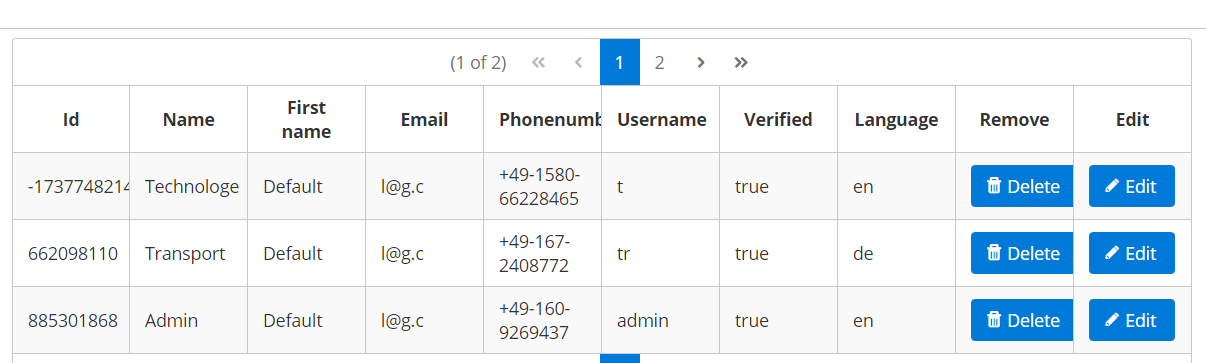
\includegraphics[width=\textwidth]{screenshots/admin/nutzertabelle.png}
  \caption{Nutzertabelle}
  \label{fig:boat1}
\end{center}
\end{figure}

 In dieser Tabelle können Sie durch drücken auf den Knopf Löschen den Benutzer der Zeile aus dem System entfernen.  \\
\begin{figure}[h!]
\begin{center}
 
\includegraphics[width=\textwidth]{screenshots/admin/nutzerloeschen.png}
  \caption{Nutzer erfolgreich gelöscht}
  \label{fig:boat2}
\end{center}
\end{figure}

Um Benutzer zu bearbeiten, drücken Sie auf den Knopf Bearbeiten, woraufhin die Daten des Users in das Formular oberhalb der Tabelle angezeigt werden, wo Sie Änderungen vornehmen können. \\
Bitte beachten Sie, in dem Feld Email nur Eingaben in der Form []@[].[] einzugeben, wobei die Endung länger als zwei Zeichen sein muss. Des weiteren dürfen für die Telefonnummer nur Zahlen eingegeben werden. Sollten Sie Fehler in den Eingaben machen, werden Ihnen die fehlerhaften Felder rot unterlegt. Die ID eines Benutzers können Sie nicht bearbeiten, da diese vom System verwaltet werden. \\
Mit Drücken auf Reset werden die bisher gespeicherten Daten wieder hergestellt. Mit Drücken auf Speichern können Sie Ihre Änderungen speichern. \\

//TODO Bild

Über der Tabelle befindet sich ein Formular, in dem Sie die Daten für einen neuen Benutzer eingeben können. Wenn sie alle Daten eingegeben haben, klicken Sie auf Speichern, um den Benutzer zu speichern. Die ID müssen Sie nicht selber eingeben, da sie vom System generiert wird. \\
Hier gelten die gleichen Beschränkungen wie oben für die Bearbeitung von Benutzern genannt. \\

\begin{figure}[h!]
\begin{center}
 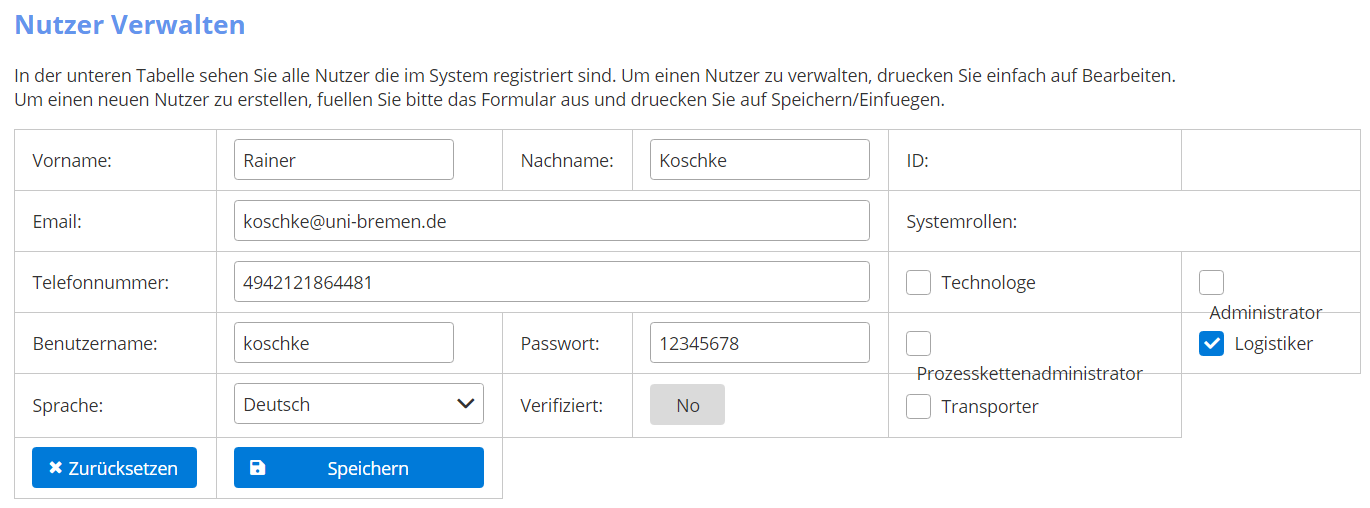
\includegraphics[width=\textwidth]{screenshots/admin/nutzerformularausgefuellt.png}
  \caption{Nutzerformular ausgefüllt}
  \label{fig:boat3}
\end{center}
\end{figure}

Bei erfolgreicher Erstellung eines Benutzer werden Sie eine Nachricht am rechten Rand des Fensters sehen, der neue Benutzer wird in der Tabelle erscheinen und eine Email bekommen. 
\begin{figure}[h!]
\begin{center}
 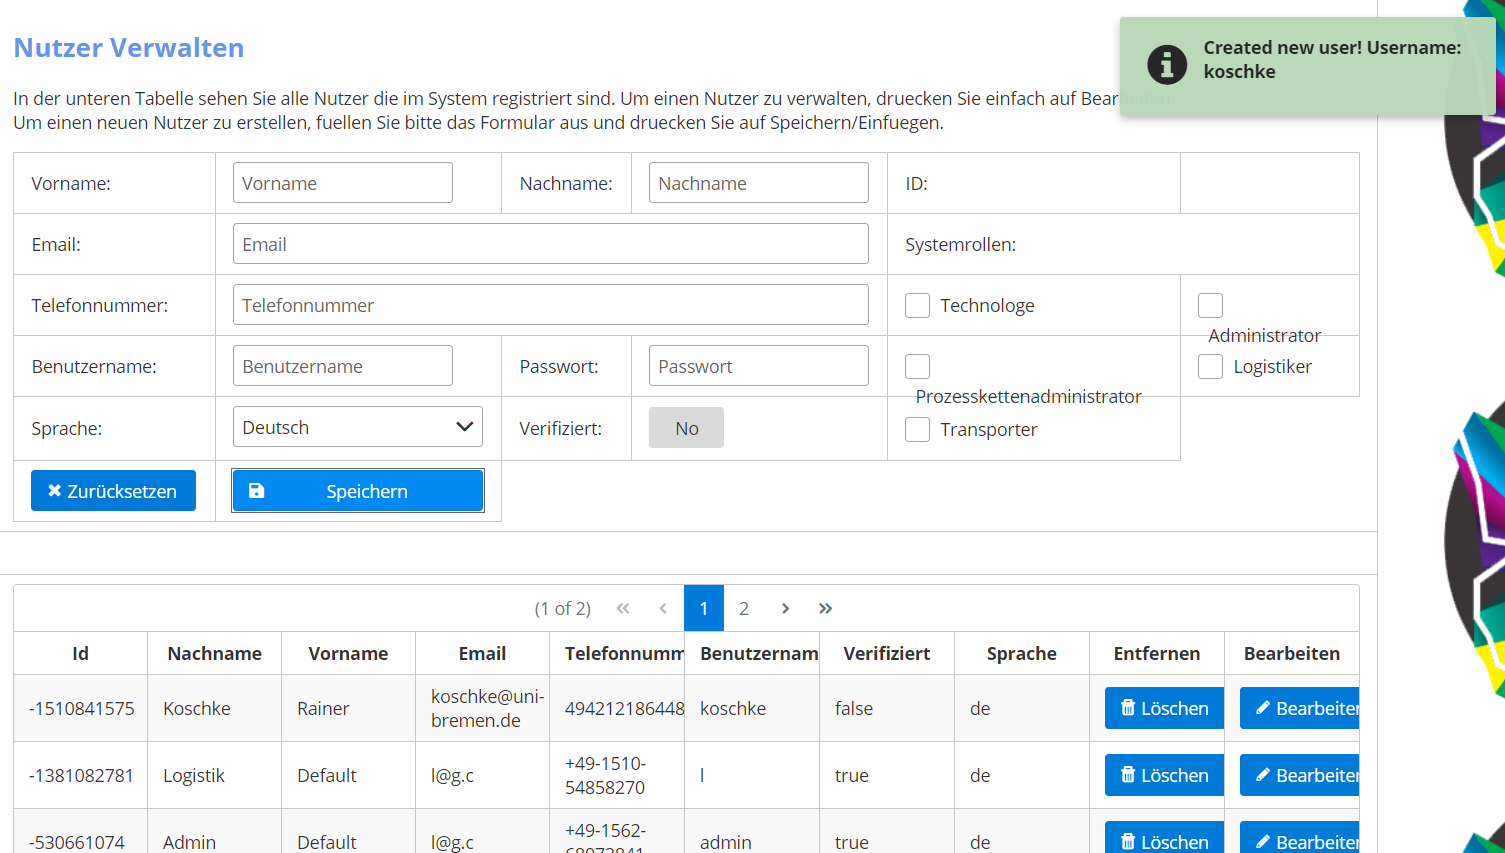
\includegraphics[width=\textwidth]{screenshots/admin/nutzererfolgreich.png}
  \caption{Nutzer erfolgreich gespeichert}
  \label{fig:boat1}
\end{center}
\end{figure}
Wenn sie die Daten im Formular zurücksetzen wollen, drücken Sie auf Reset. Dadurch werden keine Veränderungen an den vom System gespeicherten Daten vorgenommen. \\ 

\subsection{Experimentierstationen}
Die Aktionen bezüglich der Experimentierstationen können Sie unter dem Unterpunkt Experimentierstationen Verwalten im Menü aufrufen. \\
Auf der Seite sehen Sie eine Tabelle mit allen existierenden Experimentierstationen, sowie ein Formular für die Eingabe von Informationen einer Station. Die Tabelle zeigt die Stationen seitenweise an. Mithilfe der Knöpfe ober- und unterhalb der Tabelle können Sie durch die Seiten navigieren. \\

\begin{figure}[h!]
\begin{center}
 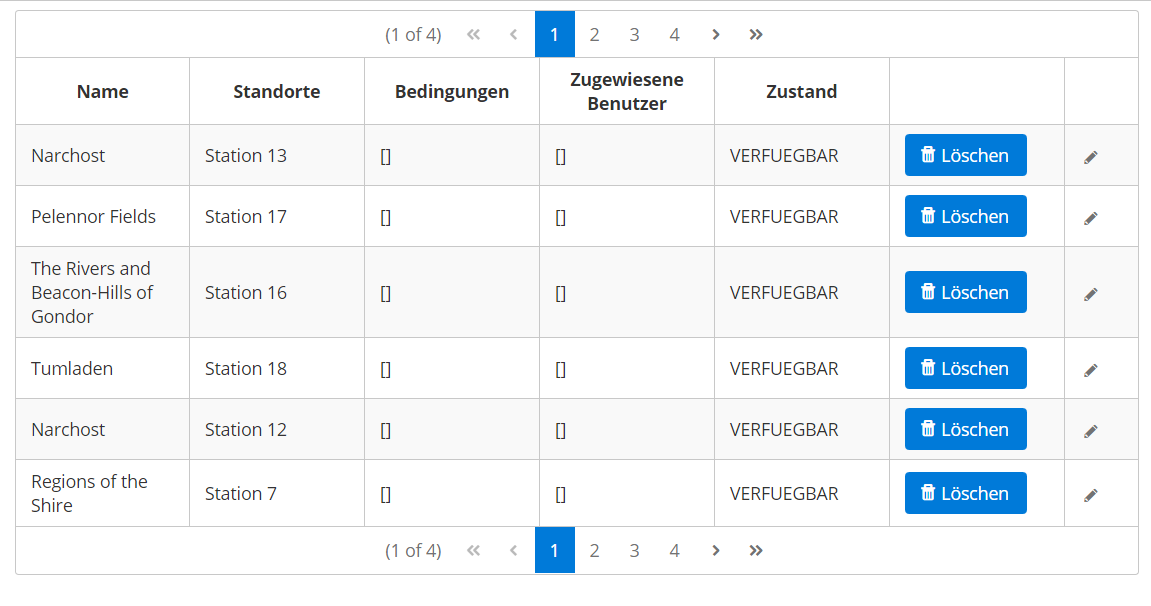
\includegraphics[width=\textwidth]{screenshots/admin/stationtabelle.png}
  \caption{Tabelle der Stationen}
  \label{fig:boat2}
\end{center}
\end{figure}

In dem Formular können Sie einen Namen eingeben, und einen Standort, die Prozessschrittparameter und die Benutzer, die an dieser Station arbeiten sollen, aussuchen. \\

\begin{figure}[h!]
\begin{center}
 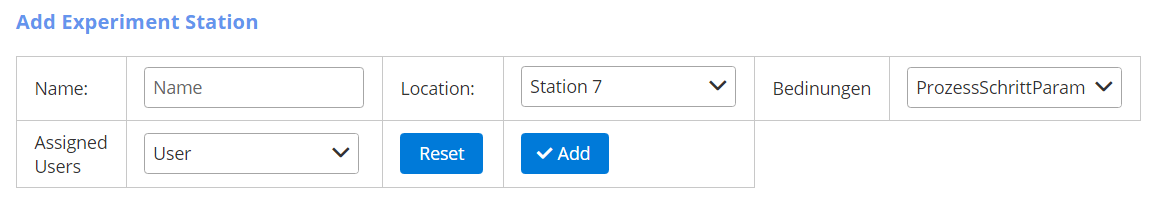
\includegraphics[width=\textwidth]{screenshots/admin/stationformular.png}
  \caption{Formular für Stationen}
  \label{fig:boat2}
\end{center}
\end{figure}

Für Benutzer, Parameter und Standort wählen Sie bitte die passenden Informationen aus der Liste, die Ihnen nach Klick auf das betreffende Feld angezeigt wird, aus. Bitte beachten Sie, dass alle Felder ausgefüllt sein müssen. \\

\begin{figure}[h!]
\begin{center}
 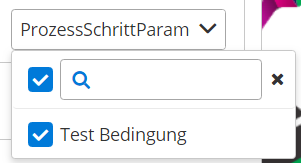
\includegraphics[width=\textwidth]{screenshots/admin/stationpsp.png}
  \caption{Prozessschrittparameter für Stationen}
  \label{fig:boat2}
\end{center}
\end{figure}

\begin{figure}[h!]
\begin{center}
 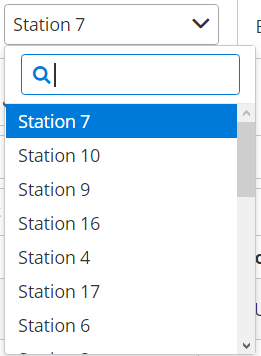
\includegraphics[width=\textwidth]{screenshots/admin/stationstandortliste.png}
  \caption{Station Standort List}
  \label{fig:boat2}
\end{center}
\end{figure}

\begin{figure}[h!]
\begin{center}
 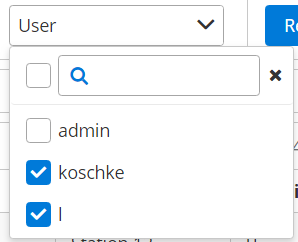
\includegraphics[width=\textwidth]{screenshots/admin/stationuser.png}
  \caption{Station Benutzer}
  \label{fig:boat2}
\end{center}
\end{figure}

Um die Station zu speichern, drücken Sie auf Erstellen, woraufhin Sie diese in der Tabelle sehen können. Um Ihre Eingaben zurückzusetzen, drücken Sie auf Zurücksetzen. \\


Wollen Sie eine existierende Station löschen, drücke Sie in der Tabellenzeile der Station auf Löschen. Die Station wird daraufhin aus der Tabelle entfernt. \\
Wenn Sie eine existierende Station bearbeiten wollen, drücken Sie in der Tabellenzeile auf den Stift. Daraufhin können Sie in die Zelle klicken, die Sie bearbeiten wollen, und dann die Informationen analog zur Eingabe im Formular auswählen. Nachdem Sie fertig sind mit der Bearbeitung der Station, klicken Sie bitte auf den Haken, der am Ende der Zeile statt des Stifts erschienen ist. Wenn Sie die Eingabe abbrechen wollen, drücken Sie auf das Kreuz. Auch hier müssen alle Felder ausgefüllt sein. \\

\begin{figure}[h!]
\begin{center}
 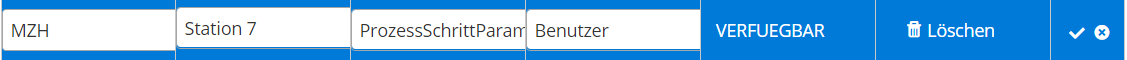
\includegraphics[width=\textwidth]{screenshots/admin/stationbearbeiten.png}
  \caption{Bearbeiten einer Station}
  \label{fig:boat2}
\end{center}
\end{figure}


%%%%%%%%%%

\subsection{Standorte}
Die Aktionen bezüglich der Standorte können Sie unter dem Unterpunkt Standort Verwalten im Menü aufrufen. \\
Auf dieser Seite sehen Sie eine Tabelle, in der alle existierenden Standorte angezeigt werden, und ein Feld, in dem Sie den Namen eines neuen Standorts eingeben können. \\

\begin{figure}[h!]
\begin{center}
 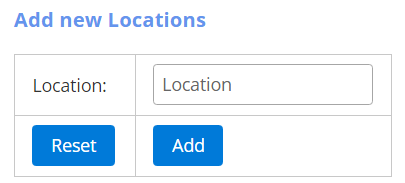
\includegraphics[width=\textwidth]{screenshots/admin/standortformular.png}
  \caption{Standort Formular}
  \label{fig:boat2}
\end{center}
\end{figure}

Um einen neuen Standort zu speichern, geben Sie einfach den Namen des Standorts in das Feld ein, und drücke Sie auf Erstellen. Nach erfolgreichem Speichern wird dieser der Tabelle hinzugefügt. \\

\begin{figure}[h!]
\begin{center}
 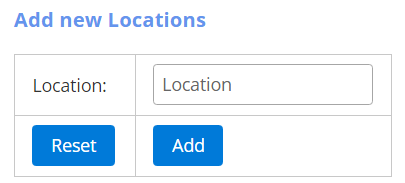
\includegraphics[width=\textwidth]{screenshots/admin/standortformular.png}
  \caption{Standortformular}
  \label{fig:boat2}
\end{center}
\end{figure}

Wenn Sie einen existierenden Standort löschen wollen, klicken Sie in der Tabellenzeile des Standorts auf Löschen. Der Standort verschwindet daraufhin aus der Tabelle. \\

Um einen existierenden Standort zu bearbeiten, klicken Sie in der entsprechenden Tabellenzeile auf das Stift Symbol. Daraufhin können Sie in die Zelle mit dem Namen klicken und diesen editieren. Wenn Sie fertig sind, klicken Sie auf den Haken, der am Ende der Zeile an der Stelle des Stifts erschienen ist. Wenn Sie den Vorgang abbrechen und auf den alten Namen zurücksetzen wollen, klicken Sie auf das Kreuz. \\

\begin{figure}[h!]
\begin{center}
 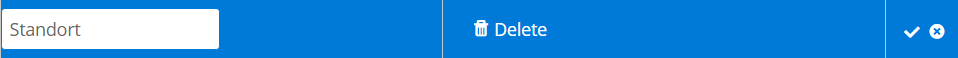
\includegraphics[width=\textwidth]{screenshots/admin/standortbearbeiten.png}
  \caption{Standort Bearbeiten}
  \label{fig:boat2}
\end{center}
\end{figure}


%%%%%%%%%%
\subsection{Globale Einstellungen}
Unter dem Unterpunkt Globale Einstellungen können Sie die Zeiten von alten Aufträgen verwalten und ändern. \\
Auf der Seite können Sie eine Tabelle sehen, die alle Aufträge beinhaltet, die bereits vollständig bearbeitet wurden. Für jeden Auftrag können Sie die Zeiten für die Erstellung, den Start, die Beendung und die Archivierung sehen. \\
Wenn Sie die Zeiten eines Auftrags bearbeiten wollen, drücken Sie auf das Stift-Symbol in der entsprechenden Zeile. Daraufhin können Sie in die Zelle klicken, die Sie bearbeiten wollen, und eine neue Zeit eingeben. Zeiten werden wie folgt eingegeben: YYYY:MM:DDTHH:MM. 
Wollen Sie Ihre Änderungen speichern, klicken Sie auf den Haken, der anstelle des Stifts erschienen ist. Wollen Sie Ihre ungespeicherten Änderungen zurücksetzen, klicken Sie auf das Kreuz neben dem Haken. \\
Bitte beachten Sie, dass für jeden Auftrag alle vier Zeiten angegeben sein müssen, und Sie keine Zeiten löschen können. \\

%%%%%%%%%%
\subsection{Backup der Systemdaten}
Unter dem Unterpunkt Backup und Wiederherstellen können Sie die aktuelle Datenbank mit all ihrer Daten exportieren, oder neue Daten aus einer existierenden Datenbank importieren. \\

Um ein Backup der Daten zu erstellen, müssen Sie nur auf Backup Erstellen klicken. Daraufhin wird ein Backup automatisch erstellt. //TODO \\

Wollen Sie Daten aus einer Datei einlesen, klicken Sie auf Choose. Daraufhin öffnet sich ein Fenster, in dem Sie aus Ihrem Dateisystem die Datei auswählen können. Wenn Sie eine Datei ausgewählt haben, drücken Sie auf Öffnen, woraufhin die Datei hochgeladen wird. Mit einem Klick auf Submit werden die Daten aus der Datei in die Datenbank integriert. Bitte beachten Sie, dass  Sie eine SQL Datei auswählen müssen. \\ 

%%%%%%%%%%%%%%%%%%%%%%%%%%%%%%%%%%%%%%%%%%%%%%%%%%%%%%%%%%%%%%%%%%%%%%%%

\newpage
\section{Farbige Zustände für andere Mitarbeiter}
\subsection{Prozesskettenadministrator}

Hier finden Sie Anleitungen für alle Aktionen, die ein Prozesskettenadministrator ausführen kann.
%%%%%%%%%%
\subsubsection{Prozessschritte}

Im Menüunterpunkt Prozessschritt haben Sie eine Übersicht über alle Prozessschritte, die aktuell im System existieren, können diese bearbeiten und löschen, sowie neue hinzufügen. Prozessschritte werden seitenweise angezeigt, Sie können durch die Seiten mithilfe der Navigatoren ober- und unterhalb der Tabelle navigieren. Bitte beachten Sie, dass Sie nur Schritte bearbeiten und löschen können, die noch nicht gestartet wurden. \\

Wenn Sie einen neuen Prozessschritt erstellen wollen, geben Sie bitte im Formular am Anfang der Seite alle Informationen für diesen ein. Dazu gehört, dass Sie eine existierende Vorlage auswählen, einen Namen eingeben, und Attribute //TODO. Bitte beachten Sie, dass Sie in allen Feldern Eingaben machen müssen. Um diesen Schritt zu speichern, drücken Sie auf Speichern. Nach der erfolgreichen Speicherung wird dieser in der Tabelle zu sehen sein. Um das Formular zurückzusetzen, drücken Sie auf Zurücksetzen; dadurch entstehen keine Änderungen am Datensatz im System. \\

\begin{figure}[h!]
\begin{center}
 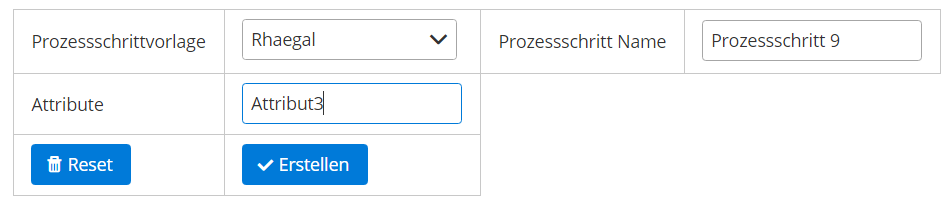
\includegraphics[width=\textwidth]{screenshots/pk/01prozessschrittformular.png}
  \caption{Das Formular für neue Prozessschritte}
  \label{fig:boat2}
\end{center}
\end{figure}


Wenn Sie einen existierenden Prozessschritt bearbeiten wollen, drücken Sie in der Zeile, in der der gewünschte Schritt in der Tabelle steht, auf das Stift-Symbol. Danach können Sie in die Zelle, die Sie bearbeiten wollen, klicken, und die Änderungen vornehmen. Bitte beachten Sie, dass Sie den Status, die Parameter und den Log nicht bearbeiten können. Wenn Sie fertig mit Ihren Änderungen sind, drücken Sie auf den Haken, der an der Stelle des Stifts erschienen ist. Wenn Sie ungespeicherte Änderungen zurücksetzen wollen, drücken Sie auf das Kreuz; dadurch werden die Daten für den Prozessschritt auf den aktuellen Stand in der Datenbank gesetzt. \\


Wollen Sie einen Prozessschritt löschen, drücken Sie auf das Löschen Symbol in der Zeile des Schrittes, den Sie löschen wollen. \\

//TODO Logs, Parameter anzeigen
%%%%%%%%%%
\subsubsection{Prozessschritt Vorlage}

Im Menü-Unterpunkt Prozessschritt Vorlage haben Sie eine Übersicht über alle in der Datenbank existierenden Prozessschritt Vorlagen, können diese bearbeiten und Löschen, sowie neue hinzufügen. \\

Um eine neue Vorlage zu speichern, geben Sie bitte in das Formular alle Informationen ein. Dafür müssen Sie aus den bestehenden Parametern alle, die hier zutreffen, die richtige Zustandsautomat Vorlage, und die Experimentierstationen, an denen dieser Schritt ausgeführt werden kann, auswählen, sowie die Dauer, die dieser Schritt vorraussichtlich haben wird und den Namen der neuen Vorlage eingeben. Zusätzlich müssen Sie auswählen, ob der Schritt Urformend sein wird, das heißt, ob durch die Ausführung des Schrittes neue Proben entstehen. Wenn der Prozessschritt urformend sein soll, geben Sie bitte im Feld daneben die Anzahl an Proben an, die erstellt werden. Bitte beachten Sie, dass Sie für alle Felder Angaben machen müssen. Die Dauer muss von der Form xx:xx sein, und darf nicht 23:59 überschreiten. Um die neue Vorlage zu speichern, drücken Sie auf Erstellen. Danach wird die neue Vorlage in der Tabelle angezeigt. Wenn Sie Ihre Eingaben löschen wollen, drücken Sie auf Zurücksetzen, dadurch werden keine Veränderungen an den Daten in der Datenbank vorgenommen. \\

\begin{figure}[h!]
\begin{center}
 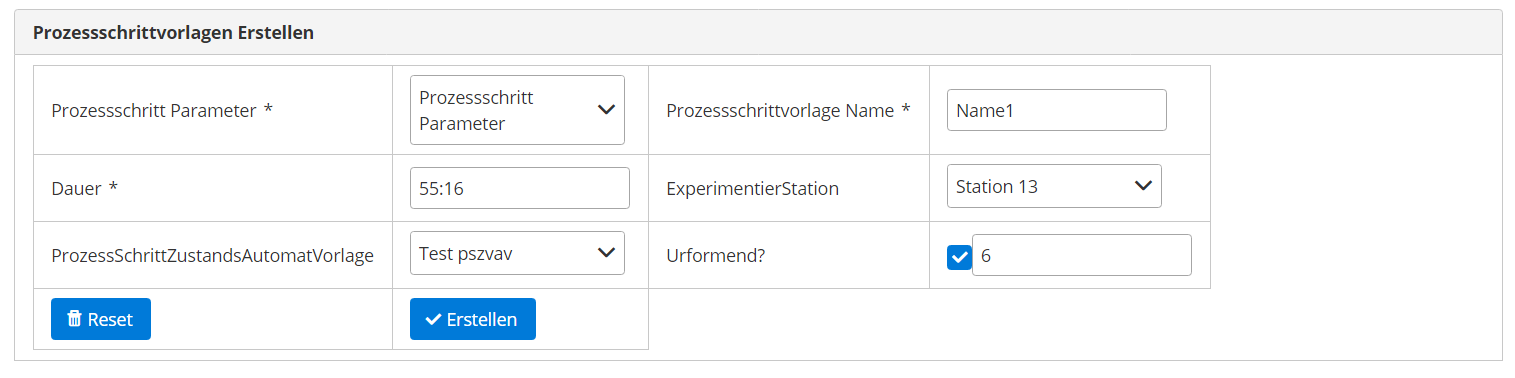
\includegraphics[width=\textwidth]{screenshots/pk/prozessschrittvorlageformular.png}
  \caption{Das Formular für eine neue Prozessschrittvorlage}
  \label{fig:boat2}
\end{center}
\end{figure}

\begin{figure}[h!]
\begin{center}
 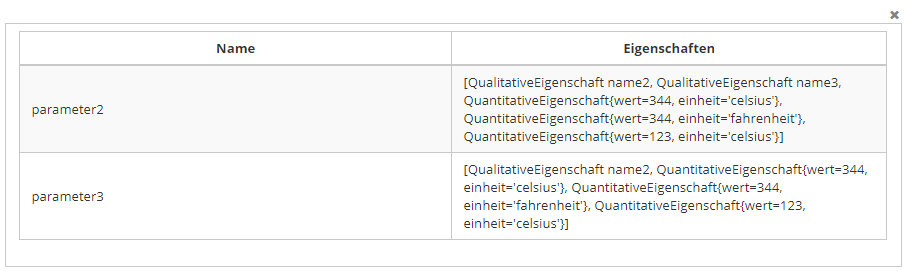
\includegraphics[width=\textwidth]{screenshots/pk/prozessschrittvorlageparameter.png}
  \caption{Auswählen von Parametern für Prozessschritt Vorlagen}
  \label{fig:boat2}
\end{center}
\end{figure}


Für die Bearbeitung von einer Vorlage drücken Sie in der entsprechenden Tabellenzeile auf das Stift-Symbol. Danach können Sie in die Zellen klicken, die Sie bearbeiten wollen, und die entsprechenden Änderungen machen. Um Ihre Änderungen zu speichern, drücken Sie auf den Haken, der an der Stelle des Stifts erschienen ist. Durch Drücken auf das Kreuz können Sie Ihre Änderungen zurücksetzen auf die Daten, die in der Datenbank gespeichert sind. \\

\begin{figure}[h!]
\begin{center}
 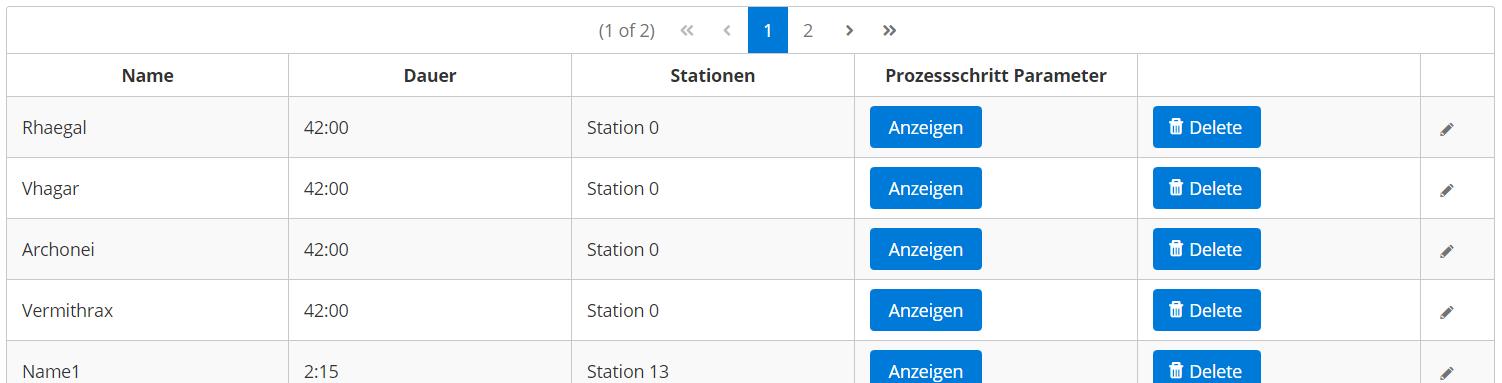
\includegraphics[width=\textwidth]{screenshots/pk/prozessschrittvorlagetabelle.png}
  \caption{Die Tabelle für die Prozessschritt Vorlagen}
  \label{fig:boat2}
\end{center}
\end{figure}


Wollen Sie eine Vorlage löschen, drücken Sie in der entsprechenden Tabellenzeile auf Löschen. \\


%%%%%%%%%%
\subsubsection{Prozessschritt Zustandsautomat}

Im Menü-Unterpunkt Prozessschrittzustandsautomatvorlagen Verwaltung haben Sie eine Übersicht über alle in der Datenbank existierenden Prozessschrittzustandsautomatvorlagen, können diese bearbeiten und löschen, sowie neue hinzufügen. \\
In der Tabelle der aktuell in der Datenbank gespeicherten Vorlagen können Sie mit den Navigatoren ober- und unterhalb der Tabelle zwischen den Seiten navigieren, alle Felder durch das Suchfeld \"Search all fields\" nach Schlagwörtern durchsuchen, ebenso sowie die Spalten Name und Zustandsreihenfolge durch die Suchfelder in den jeweiligen Spalten. \\
Durch die Felder in der ganz linken Spalte der Tabelle können Sie Vorlagen auswählen, um //TODO \\

\begin{figure}[h!]
\begin{center}
 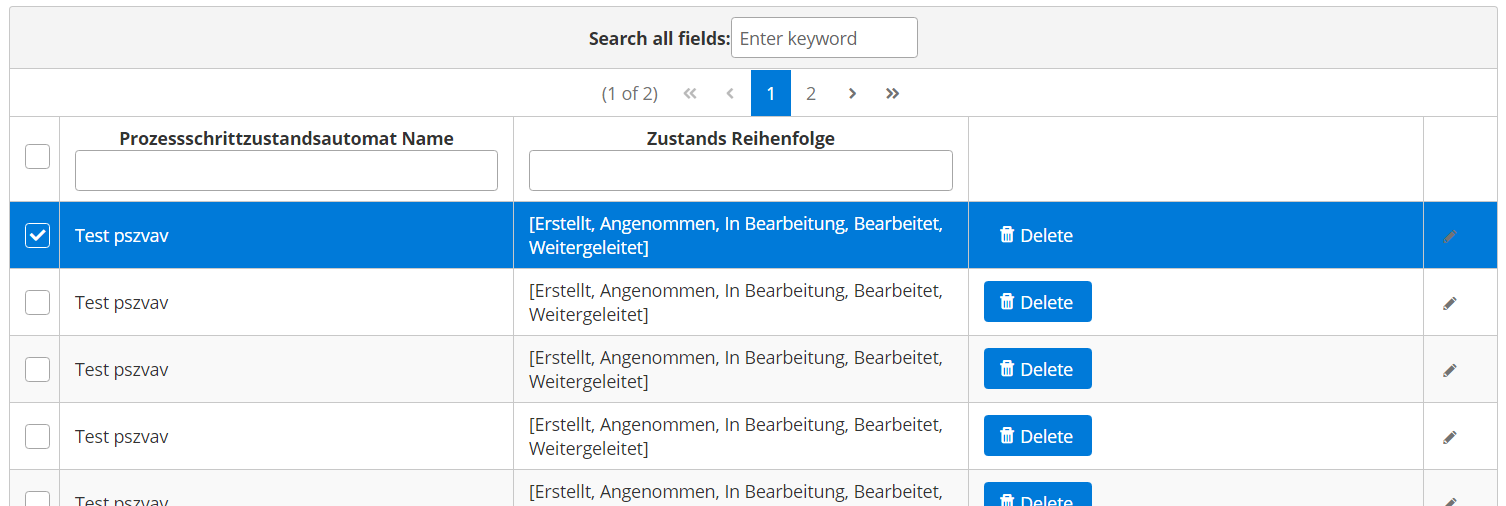
\includegraphics[width=\textwidth]{screenshots/pk/zustandsautomattabelle.png}
  \caption{Tabelle für die Zustandsautomat Vorlagen}
  \label{fig:boat2}
\end{center}
\end{figure}

Wollen Sie einen neuen Zustandsautomat erstellen, benutzen Sie das Formular am Anfang der Seite. Dort können Sie im Eingabefeld \"Zustaende einfuegen\" den Namen eines neuen Zustands eingeben, und Ihn durch Klicken auf Einfuegen in die Liste an Zuständen in der Anzeige "Zustandsautomat Erstellen" einfügen. Dort wird er auf der linken Seite am Ende der dort bereits stehenden Liste erscheinen. In dieser Anzeige können Sie die Zustände mit den Rechts- und Linkspfeilen zwischen dem rechten und linken Feld hin-und herschieben, wo sie jeweils am Ende der List stehen werden. Die doppelten Pfeile bewegen alle Zustände von einer Seite zu der anderen und behalten dabei die Reihenfolge, in der Sie in Ihrem ursprünglichen Feld standen. Sie müssen die Zustände in der richtigen Reihenfolge auf der rechten Seite sortieren. In der unteren Zeile können Sie einen Namen für Ihre neuen Zustandsautomatenvorlage eingeben. Bitte beachten Sie, dass jede Vorlage einen Zustand Erstellt enthalten muss, der am Anfang des Zustandsautomat steht. 
Nachdem Sie die Zustände auf der rechten Seite richtig stehen haben und einen Namen haben, können Sie auf Erstellen drücken, um die Vorlage zu erstellen, und in die Tabelle der existierenden Vorlagen einzufügen. Durch Drücken auf Zurücksetzen können Sie im Formular Ihre Änderungen löschen, wodurch keine Änderungen an den Daten in der Datenbank entstehen. \\

\begin{figure}[h!]
\begin{center}
 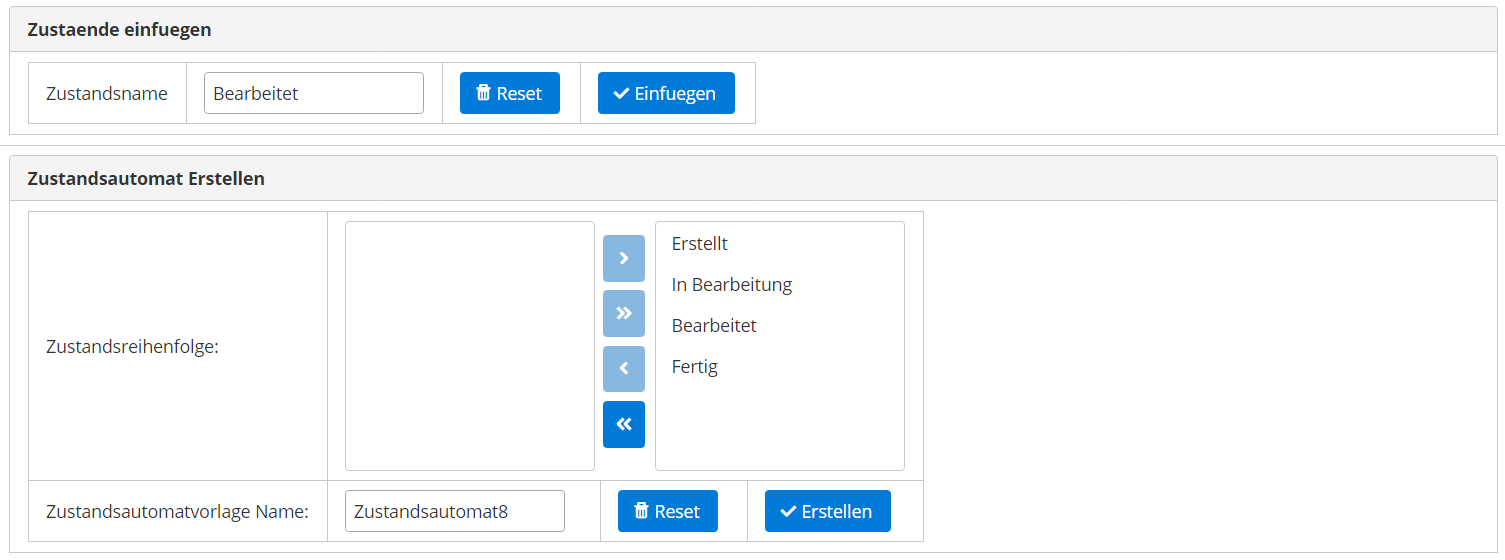
\includegraphics[width=\textwidth]{screenshots/pk/zustandsautomatformular.png}
  \caption{Formular für neue Zustandsautomat Vorlagen}
  \label{fig:boat2}
\end{center}
\end{figure}


Wenn Sie eine Zustandsautomatvorlage löschen wollen, drücken Sie auf Löschen in der entsprechenden Tabellenzeile. Dadurch wird die Vorlage aus der Datenbank entfernt, und kann nicht wieder hergestellt werden. \\


Um eine Vorlage zu bearbeiten, drücken Sie in der Tabellenzeile der gewünschten Vorlage auf das Stift-Symbol. Danach können Sie die gewünschten Änderungen eingeben, wobei das Bewegen der Zustände mit den Pfeiltasten zwischen den beiden Feldern ermöglicht wird. Die richtige Zustandsreihenfolge soll am Ende auf der rechten Seite stehen. Nachdem Sie alle gewünschten Änderungen gemacht haben, drücken Sie auf den Haken, der an Stelle des Stifts erschienen ist, wodurch diese gespeichert werden. Wenn Sie die Änderungen verwerfen und die Daten auf die in der Datenbank gespeicherten zurücksetzen wollen, drücken Sie auf das Kreuz. \\

\begin{figure}[h!]
\begin{center}
 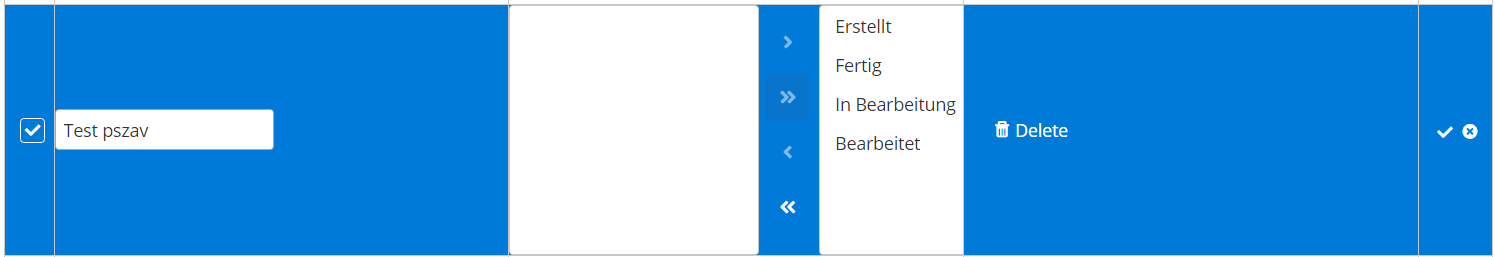
\includegraphics[width=\textwidth]{screenshots/pk/zustandsautomatbearbeiten.png}
  \caption{Bearbeiten einer Zustandsautomat Vorlage}
  \label{fig:boat2}
\end{center}
\end{figure}

%%%%%%%%%%
\subsubsection{Prozessschritt Parameter}
%%%%%%%%%%
\subsubsection{Prozessketten Vorlagen}
%%%%%%%%%%
\subsubsection{Aufträge}
%%%%%%%%%%
\subsubsection{Qualitative/Quantitative Eigenschaften}
%%%%%%%%%%
\subsubsection{Arbeitsauslastung}
%%%%%%%%%%
\subsubsection{JSON Export}
%%%%%%%%%%
\subsection{Logistiker}
\subsubsection{Übersicht über Träger}
\subsubsection{Übersicht über freigegeben Aufträge}
\subsubsection{Übersicht über Probenmengen}
\subsubsection{Übersicht über archivierte Proben}
\subsubsection{Übersicht über Probenstandorte}
\subsection{Technologe}
\subsubsection{Übersicht über Experimentierstationen}
\subsubsection{Übersicht über aktuelle Arbeitsarufträge}
\subsubsection{Übersicht über angekündigte Abeitsaufträge}
\subsubsection{Aktualisieren des Zustands eines Arbeitrauftrags}
\subsubsection{Probenupload}
\subsubsection{Proben melden}
\subsubsection{Experimentierstation melden}
\subsubsection{Kommentare}
\subsection{Transporter}
\subsubsection{Übersicht über anstehende Transportaufträge}
\subsubsection{Probenverlust melden}

%%%%%%%%%%%%%%%%%%%%%%%%%%%%%%%%%%%%%%%%%%%%%%%%%%%%%%%%%%%%%%%%%%%%%%%%

\newpage
\section{Probleme und Ursachen}

%%%%%%%%%%%%%%%%%%%%%%%%%%%%%%%%%%%%%%%%%%%%%%%%%%%%%%%%%%%%%%%%%%%%%%%%

\end{document}